\documentclass[12pt]{article}

\usepackage[utf8]{inputenc}
\usepackage{amsfonts}
\usepackage{float, graphicx}
\graphicspath{{images/}}

\usepackage{hyperref}
\hypersetup{
    pdftitle={devopspractical},
    }

\usepackage{geometry}
 \geometry{
 a4paper,
 left=3.5 cm,
 top=2.5 cm,
 right = 1.25 cm,
 bottom = 1.25 cm
 }
 
\usepackage[nottoc]{tocbibind}

\usepackage{tabularx}

\setlength{\parindent}{0 pt}

\begin{document}
\begin{titlepage}
 \centering
 

{\large \bfseries \uppercase{DevOps: Software Architecture Lab}}
\vspace{3\baselineskip}
 
{\large \uppercase{Practical File}}\\
 \vspace{2\baselineskip}
{\bfseries Bachelor of technology}
\vspace{2\baselineskip}
 
Information Technology
\vspace{4\baselineskip}

April, 2022\\
\vspace{2\baselineskip}

\begin{figure}[h]
\centering

\includegraphics[scale=0.7]{gndeclogo}
\vspace{0.6\baselineskip}
\end{figure}

\vspace{1\baselineskip}

%\begin{tabularx}{0.8\textwidth} { 
%   >{\raggedright\arraybackslash}X
%   >{\raggedright\arraybackslash}X  }
% item 11 & item 12  \\
% \vspace{1 \baselineskip}
% item 21  & item 22   \\
%\vspace{1 \baselineskip}
%\end{tabularx}

\hskip4em
\begin{tabular}{m{18em} m{15em}}

\large {\textbf{Submitted by} } & {\large \textbf{Submitted to}} \\
\vspace{0.5\baselineskip}
Parvesh Bhatt     &	\vspace{0.5\baselineskip} Prof. Harjot Kaur Gill \\
\vspace{0.5\baselineskip} 
University Roll No. 1905375   &  \\
\vspace{0.5\baselineskip}
Class Roll no. 1921078\\ &

\end{tabular}

\vspace{3\baselineskip}





\uppercase{Guru Nanak Dev Engineering college\\
Ludhiana-141006, India}
\thispagestyle{empty}
\end{titlepage}
\clearpage
\tableofcontents
\thispagestyle{empty}
\clearpage


\section{PRACTICAL 1}
\setcounter{page}{1}
{\bfseries INSTALLATION OF GIT}
\subsection{Checking for git}
To see if you already have Git installed, open up your terminal application
\begin{itemize}
\item If you're on a Mac, look for a command prompt application called "Terminal".
\item If you're on a Windows machine, open the windows command prompt or "Git Bash".[Figure \ref{gitversion}]
\end{itemize}

\noindent
Once you've opened your terminal application, type git version. The output will either tell you which version of Git is installed, or it will alert you that git is an unknown command. If it's an unknown command, read further and find out how to install Git.


\begin{figure}[H]
\centering
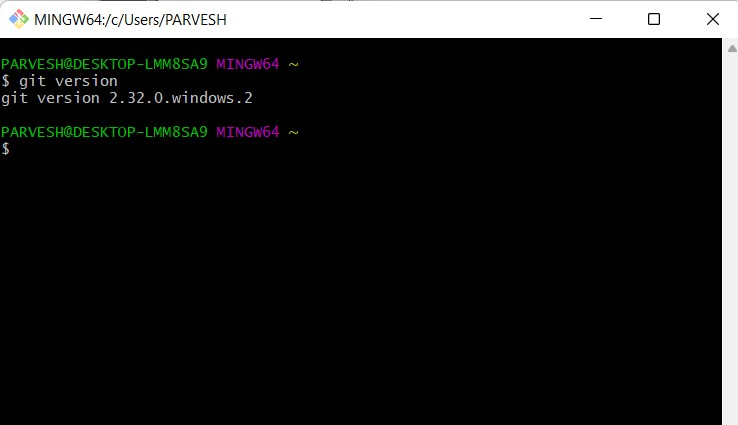
\includegraphics[scale=1]{gitversion}
\caption{Checking git version}
\label{gitversion}
\vspace{0.6\baselineskip}
\end{figure}

\subsection{Install git on Windows}
\begin{enumerate}
\item Browse to the official Git website: \href{https://git-scm.com/downloads}{https://git-scm.com/downloads}
\begin{figure}[H]
\centering
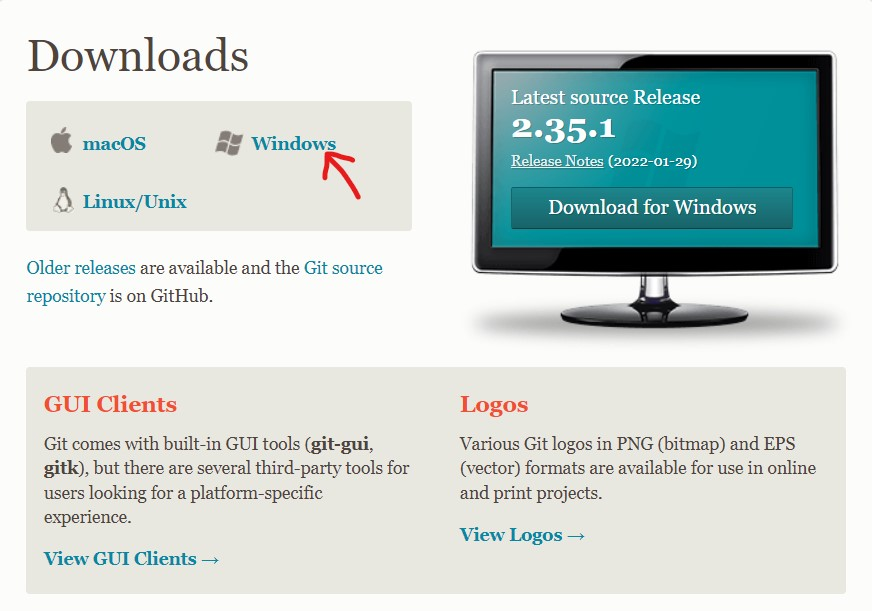
\includegraphics[scale=0.7]{gitinstallsite}
\caption{Install git site}
\label{gitversion}
\vspace{0.6\baselineskip}
\end{figure}

\item  Click the download link for Windows and allow the download to complete.

\item  Browse to the download location (or use the download shortcut in your browser). Double-click the file to extract and launch the installer.

\item Allow the app to make changes to your device by clicking Yes on the User Account Control dialog that opens.


\begin{figure}[H]
\centering
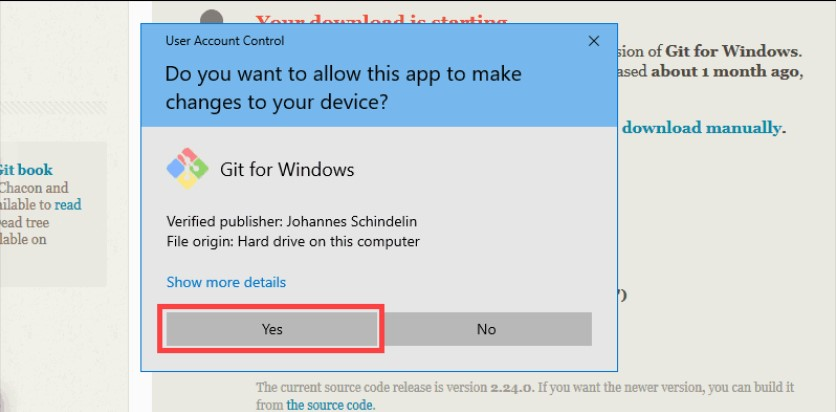
\includegraphics[scale=0.7]{gitinstall4}
\caption{Install git site}
\label{gitversion}
\vspace{0.6\baselineskip}
\end{figure}

\item Review the GNU General Public License, and when you’re ready to install, click Next.

\item The installer will ask you for an installation location. Leave the default, unless you have reason to change it, and click Next.

\begin{figure}[H]
\centering
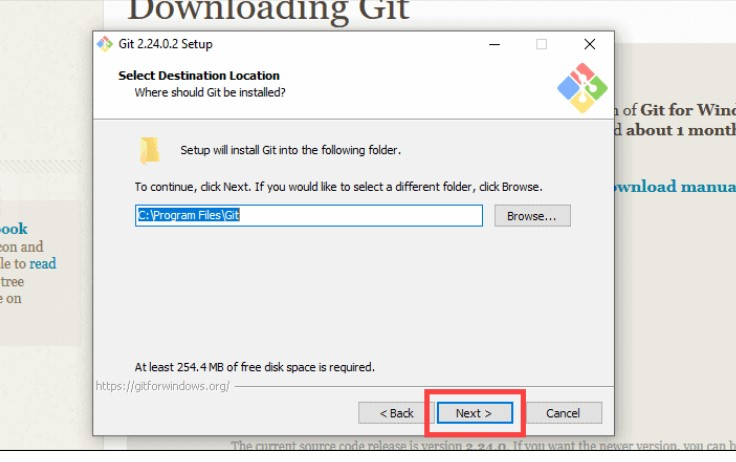
\includegraphics[scale=0.7]{gitinstall5}
\caption{Select install location}
\label{gitversion}
\vspace{0.6\baselineskip}
\end{figure}

\item A component selection screen will appear. Leave the defaults unless you have a specific need to change them and click Next.

\item The installer will offer to create a start menu folder. Simply click Next.

\item Select a text editor you’d like to use with Git. Use the drop-down menu to select Notepad++ (or whichever text editor you prefer) and click Next.

\item The next step allows you to choose a different name for your initial branch. The default is 'master.' Unless you're working in a team that requires a different name, leave the default option and click Next.

\item This installation step allows you to change the PATH environment. The PATH is the default set of directories included when you run a command from the command line. Leave this on the middle (recommended) selection and click Next.\\
\vspace{1\baselineskip}\\
{\bfseries Server Certificates, Line Endings and Terminal Emulators}

\item The installer now asks which SSH client you want Git to use. Git already comes with its own SSH client, so if you don't need a specific one, leave the default option and click Next.

\item The next option relates to server certificates. Most users should use the default. If you’re working in an Active Directory environment, you may need to switch to Windows Store certificates. Click Next.

\item The next selection converts line endings. It is recommended that you leave the default selection. This relates to the way data is formatted and changing this option may cause problems. Click Next.

\item Choose the terminal emulator you want to use. The default MinTTY is recommended, for its features. Click Next.

\item  The installer now asks what the git pull command should do. The default option is recommended unless you specifically need to change its behavior. Click Next to continue with the installation.

\item Next you should choose which credential helper to use. Git uses credential helpers to fetch or save credentials. Leave the default option as it is the most stable one, and click Next.

\item select additional customization options and click next.

\item Once the installation is complete, tick the boxes to view the Release Notes or Launch Git Bash, then click Finish.

\begin{figure}[H]
\centering
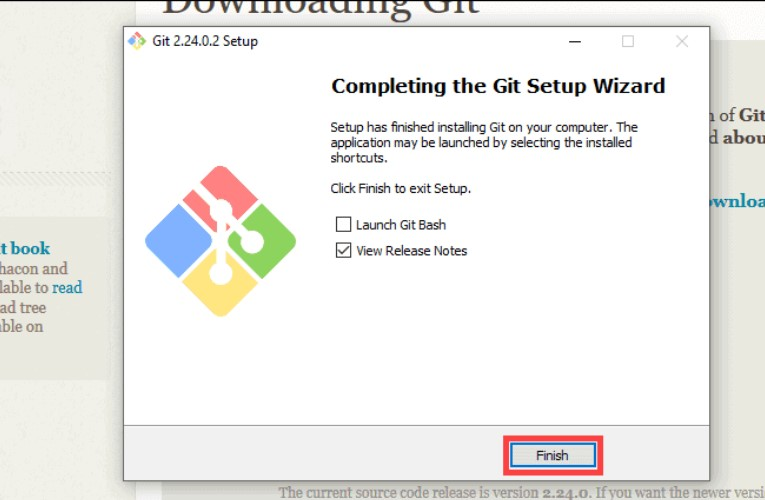
\includegraphics[scale=0.7]{gitinstall6}
\caption{Completing the git set-up wizard}
\label{gitinstall6}
\vspace{0.6\baselineskip}
\end{figure}

\end{enumerate}

\subsection{Install Git on Linux}
You can install Git on Linux through the package management tool that comes with your distribution.

\begin{enumerate}
\item Git packages are available using apt.
\item It's a good idea to make sure you're running the latest version. To do so, Navigate to your command prompt shell and run the following command to make sure everything is up-to-date: sudo apt-get update.

\item To install Git, run the following command: sudo apt-get install git-all.

\item Once the command output has completed, you can verify the installation by typing: git version.

\end{enumerate}
\clearpage


\section{PRACTICAL 2}
{\bfseries \uppercase{Create an account on github}}

\begin{enumerate}
\item  \textbf{Go to https://github.com/join in a web browser}. You can use any web browser on your
computer, phone, or tablet to join.

\item \textbf{Enter your personal details}. In addition to creating a username and entering an email address,
you'll also have to create a password. Your password must be at leas t 15 characters in length or at least 8 characters with at least one number and lower-case letter. 

\begin{figure}[H]
\centering
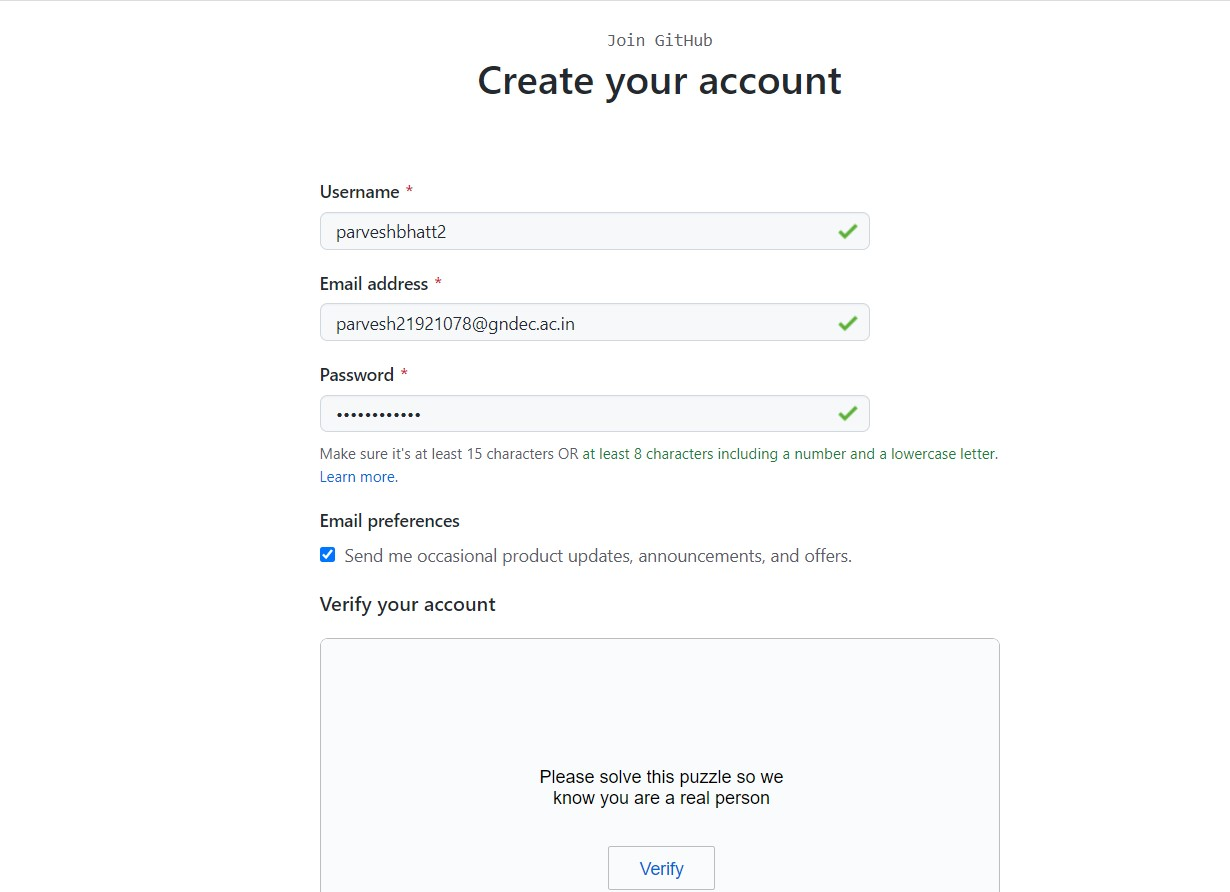
\includegraphics[scale=0.5]{p2createaccount}
\caption{Enter your personal details}
\label{gitinstall6}
\vspace{0.6\baselineskip}
\end{figure}


\item \textbf{click the green Create an account button}. It's below the form.

\item \textbf{Complete the CAPTCHA puzzle}. The instructions vary by puzzle, so just follow the on screen instructions to confirm that you are a human.

\item \textbf{Click the Choose button for your desired plan}. Once you select a plan, GitHub will send an email confirmation message to the address you entered.

\item \textbf{Click the Verify email address button in the message from GitHub}. This confirms your email address and returns you to the sign up process.

\item \textbf{Review your plan selection and click Continue}. You can also choose whether you want to receive updates from GitHub via email by checking or unchecking the "Send me updates" box.

\item \textbf{your preferences and click Submit} GitHub displays a quick survey that can help you
tailor your experience to match what you're looking for. Once you make your selection, you'll be taken to a screen that allows you to set up your first repository.

Congratulation your account on GitHub is created Successfully. Now you are
free to do your work.

\end{enumerate}


\section{PRACTICAL 3}

\textbf{\uppercase {Create Repository using GIT/ GITHUB}} \\
\vspace{0.6\baselineskip} \\
\noindent
GITHUB
\vspace{0.6\baselineskip}
\begin{enumerate}

\item In the upper-right corner of any page, use the drop-down menu, and
select New repository.

\begin{figure}[H]
\centering
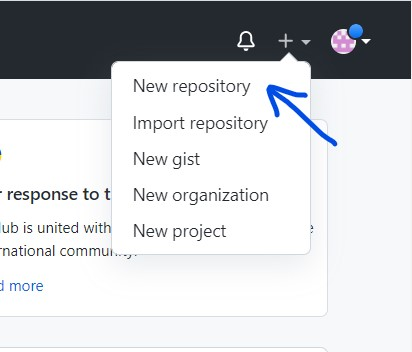
\includegraphics[scale=1]{p3(1)}
\caption{Select new repository}
\label{p3(1)}
\vspace{0.6\baselineskip}
\end{figure}


\item Type a short, memorable name for new repository. For example, "hello-devops".

\begin{figure}[H]
\centering
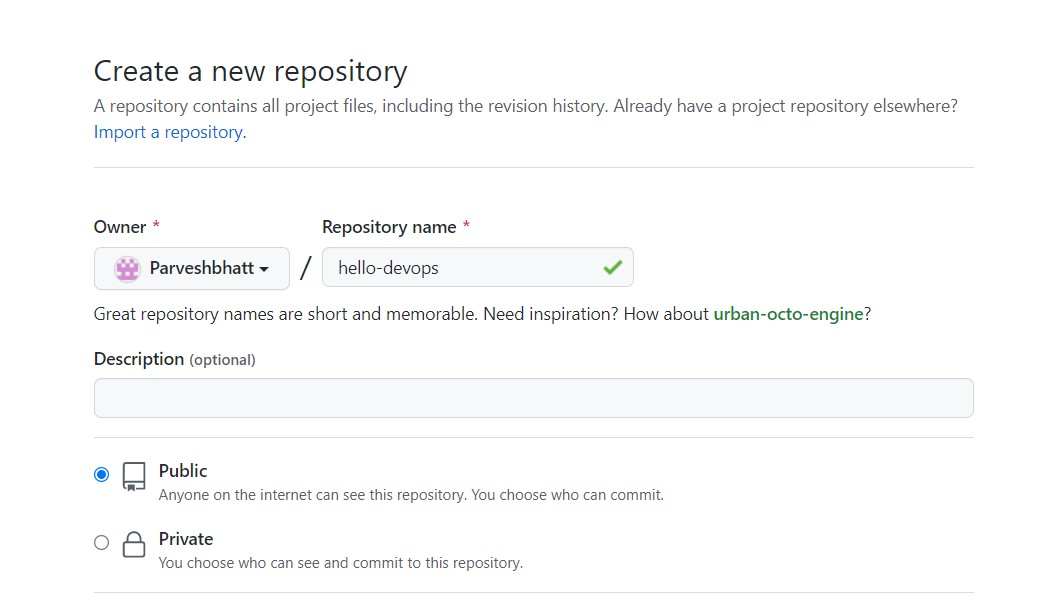
\includegraphics[scale=0.6]{p3two}
\caption{Name the repository}
\label{p3two}
\vspace{0.6\baselineskip}
\end{figure}

\item Optionally, add a description of our repository. For example, "First devops repository."

\begin{figure}[H]
\centering
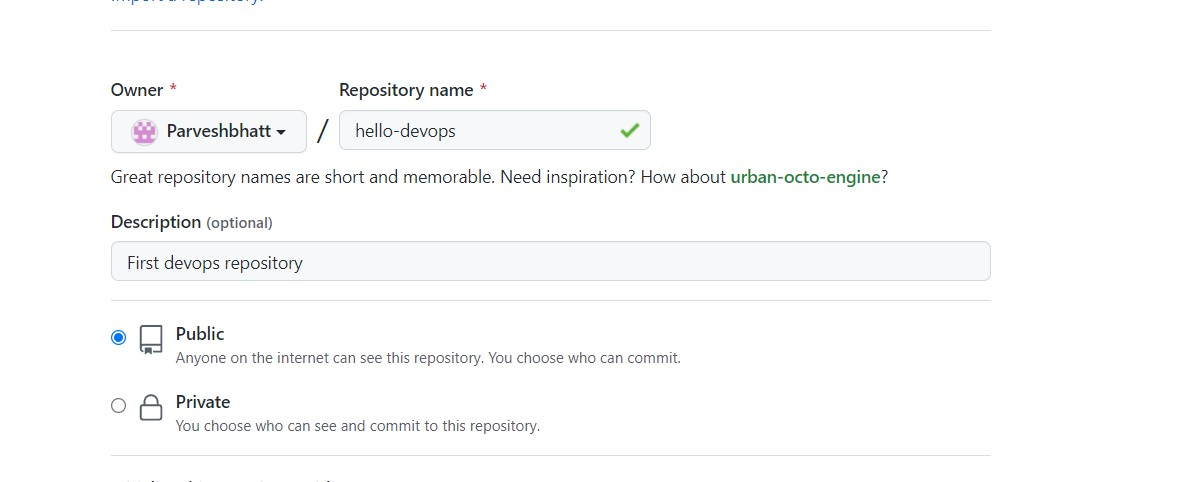
\includegraphics[scale=0.8]{p3three}
\caption{Name the repository}
\label{p3three}
\vspace{0.6\baselineskip}
\end{figure}

\item Choose a repository visibility. For more information, see \href{https://docs.github.com/en/repositories/creating-and-managing-repositories/about-repositories}{"About repositories"}.

\item Select Initialize this repository with a README.
\begin{figure}[H]
\centering
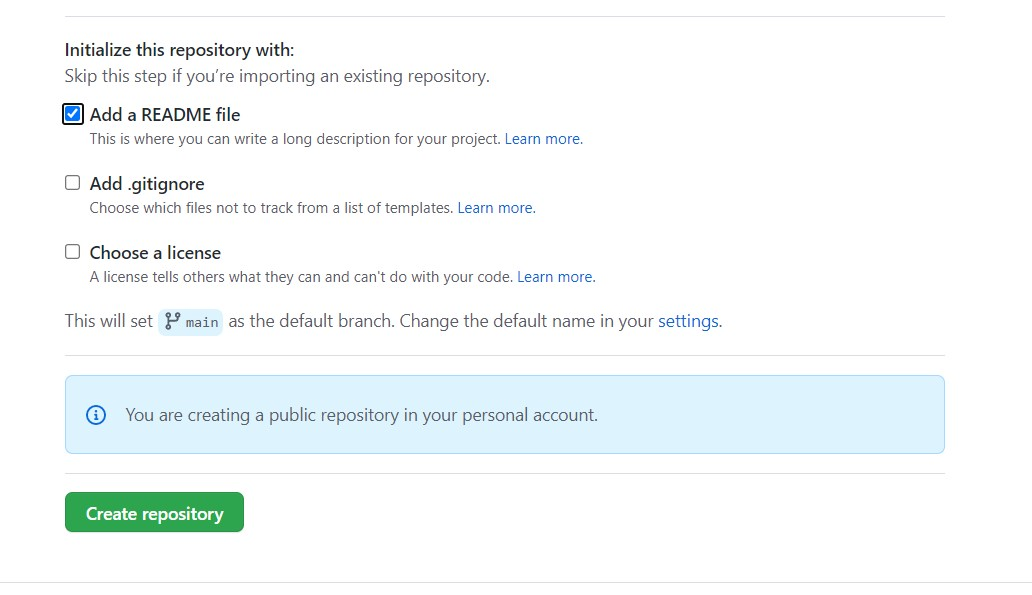
\includegraphics[scale=0.8]{p3four}
\caption{Select Add a README file}
\label{p3four}
\vspace{0.6\baselineskip}
\end{figure}

\item Click Create repository.

\end{enumerate}



\section{PRACTICAL 4}

\textbf{\uppercase {Create/Delete/Merge Branches}} \\
\vspace{0.1\baselineskip} \\
 
\subsection{CREATE BRANCH}
A new branch can be created  with the help of the \emph{git branch} command.\\

\vspace{1 mm}

\textit{\textbf{\$ git branch fix-code}}\\

\vspace{1 mm}

where fix-code is the name of new branch.

\subsection{MERGE BRANCH}
Git allows you to merge the other branch with the currently active branch. You can merge two branches with the help of \emph{git merge} command. Below command is used to merge the branches:\\

\vspace{1 mm}

For merging a branch to master or any other branch, switch over to that branch using \emph{git checkout} command.\\
\vspace{1 mm}

\textit{\textbf{\$ git checkout master}}\\

Merge the fix-code branch to master/main branch.\\

\vspace{1 mm}

\textit{\textbf{\$ git merge fix-code}}\\

\vspace{1 mm}

The fix-code branch is now merged with master branch .

\subsection{DELETE BRANCH}
For deleting specified branch, it is a safe operation. In this command, Git prevents you from deleting the branch if it has unmerged changes. Below is the command to do this.\\

\vspace{1 mm}

\textit{\textbf{\$ git branch -d fix-code}}\\

Attempting to delete an unmerged branch results in following error message.\\

\vspace{1 mm}

\textit{error: The branch 'new' is not fully merged.
If you are sure you want to delete it, run 'git branch -D new'.}\\

\vspace{1 mm}

To delete unmerged branch use same command with -D flag.\\

\vspace{1mm}

\textit{\textbf{\$ git branch -D branchname}}\\

\vspace{1mm}

For deleting a remote branch from Git desktop application. Below command is used to delete a remote branch:.\\
\vspace{1 mm}

\textit{\textbf{\$ git push origin -delete remote-branch}}\\

\clearpage

\section{PRACTICAL 5}

\textbf{\uppercase {Install Docker}} \\
\vspace{0.1\baselineskip} \\

Following are the steps to install Docker: -

\begin{enumerate}
	\item Browse to official Docker website  \href{https://docs.docker.com/desktop/windows/install/}{https://docs.docker.com/desktop/windows/install/}
	\item Double-click Docker Desktop Installer.exe to run the installer. If you haven’t already downloaded the installer (Docker Desktop Installer.exe), you can get it from Docker Hub. It typically downloads to your Downloads folder, or you can run it from the recent downloads bar at the bottom of your web browser.

\begin{figure}[H]
\centering
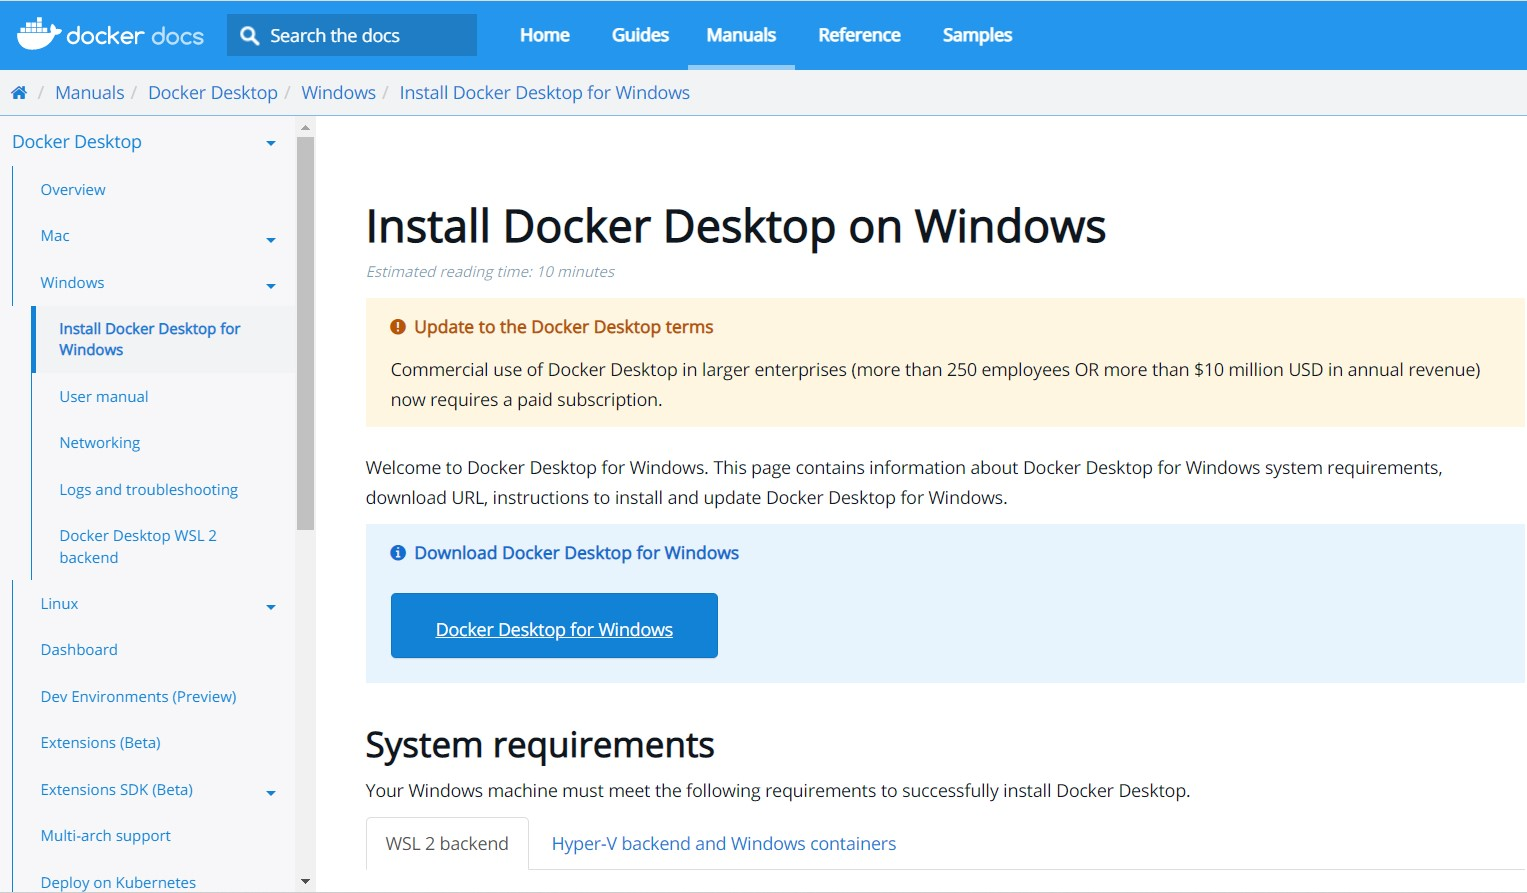
\includegraphics[scale=0.5]{fig11}
\caption{docker website}
\vspace{0.6\baselineskip}
\end{figure}	
	
	
	\item When prompted, ensure the Use WSL 2 instead of Hyper-V option on the Configuration page is selected or not depending on your choice of back-end.
	
	\item Follow the instructions on the installation wizard to authorize the installer and proceed with the install.
	
\begin{figure}[H]
\centering
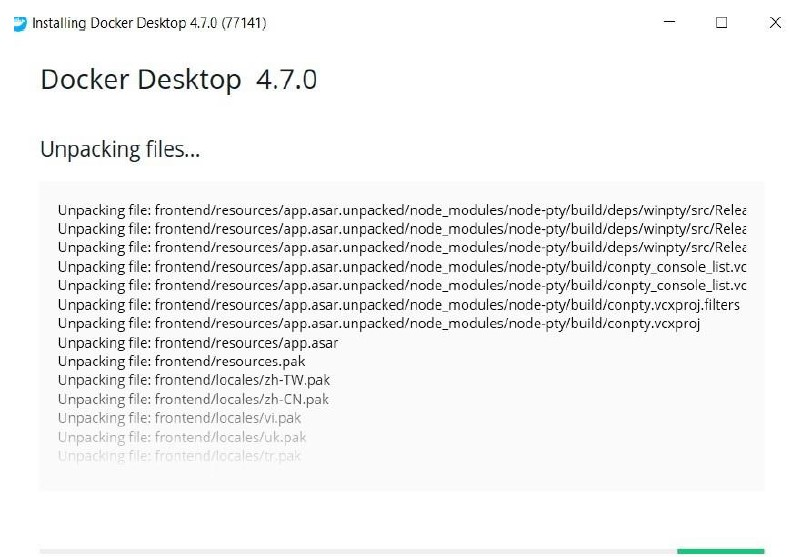
\includegraphics[scale=0.8]{fig12}
\caption{Installation wizard}
\vspace{0.6\baselineskip}
\end{figure}	
	
	\item When the installation is successful, click Close to complete the installation process.
	
\begin{figure}[H]
\centering
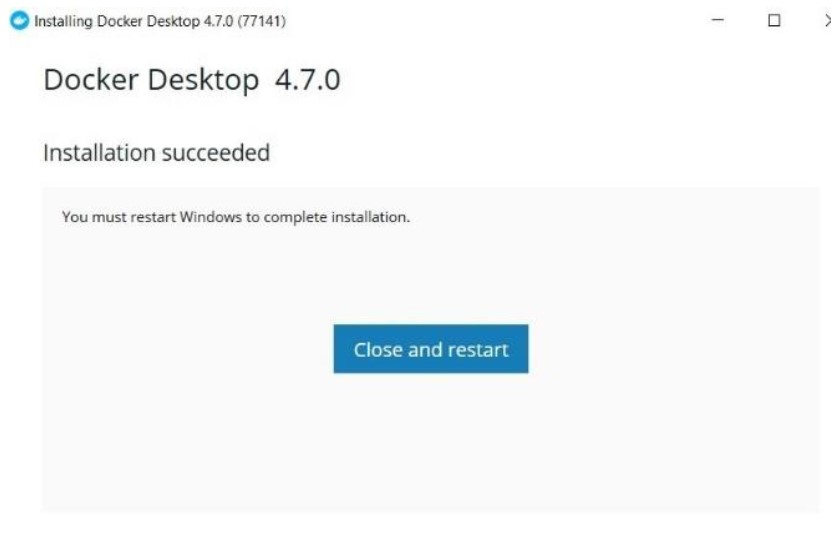
\includegraphics[scale=0.7]{fig13}
\caption{Installation Complete}
\vspace{0.6\baselineskip}
\end{figure}	
	
	\item If your admin account is different to your user account, you must add the user to the docker-users group. Run Computer Management as an administrator and navigate to Local Users and Groups ¿ Groups ¿ dockerusers. Right-click to add the user to the group. Log out and log back in for the changes to take effect

	
\begin{figure}[H]
\centering
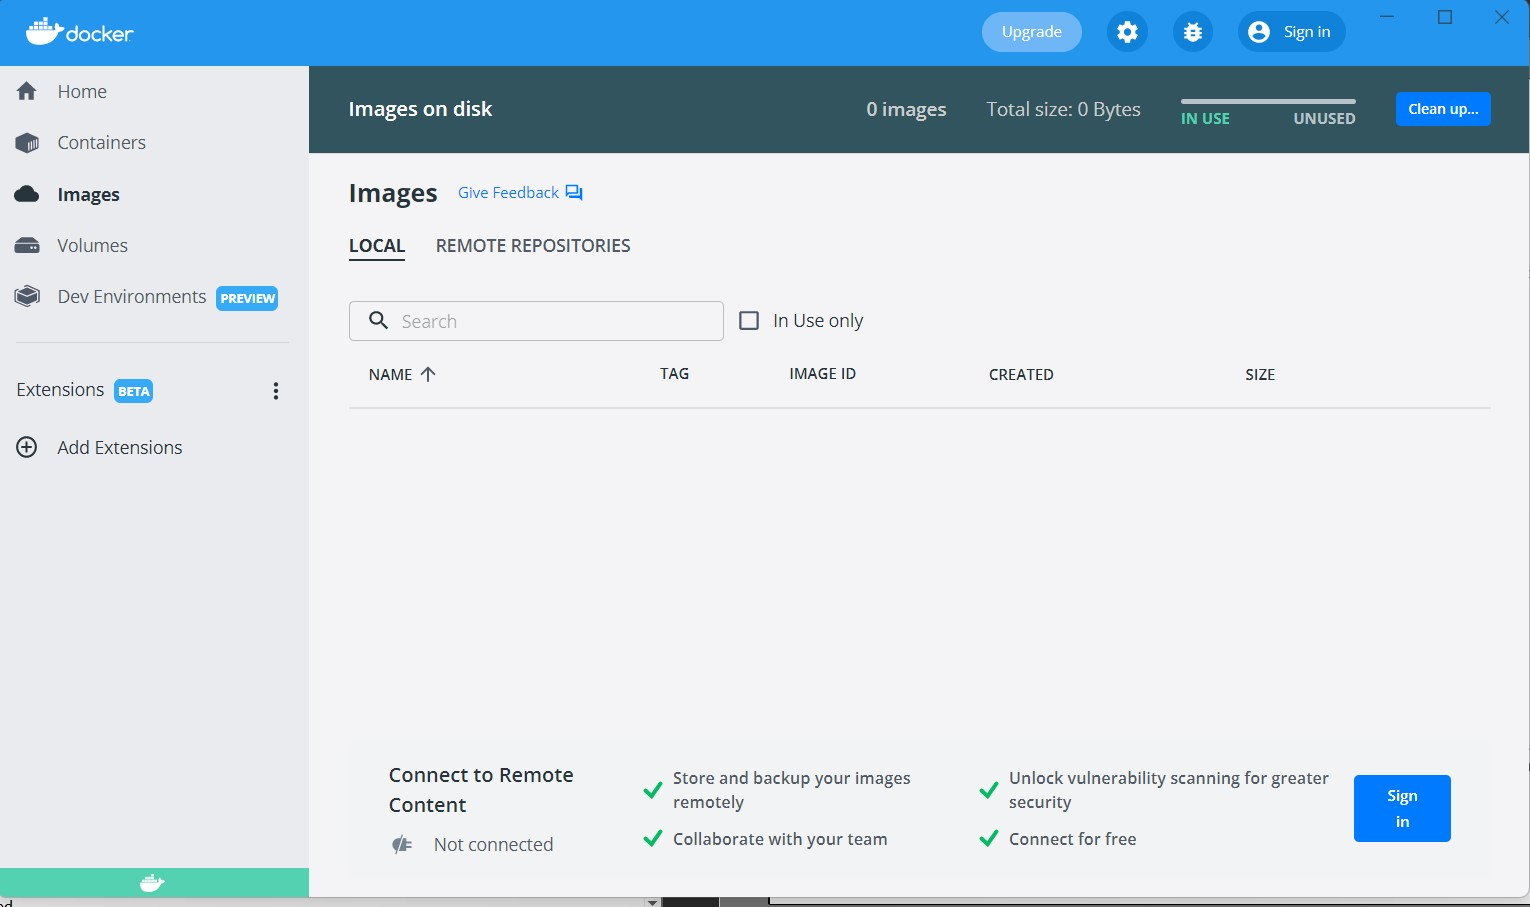
\includegraphics[scale=0.5]{fig14}
\caption{Docker Desktop}
\vspace{0.6\baselineskip}
\end{figure}	
	
\end{enumerate}

\clearpage

\section{PRACTICAL 6}

\textbf{\uppercase {Deploy Nginx Web Server Image on Docker}} \\
\vspace{0.1\baselineskip} \\

 Steps for getting the Docker container for nginx up and running.
 
 \begin{enumerate}
 \item The first step is to pull the image from Docker Hub. When you log into Docker Hub, you will be able to search and see the image for nginx as shown below.
 
\begin{figure}[H]
\centering
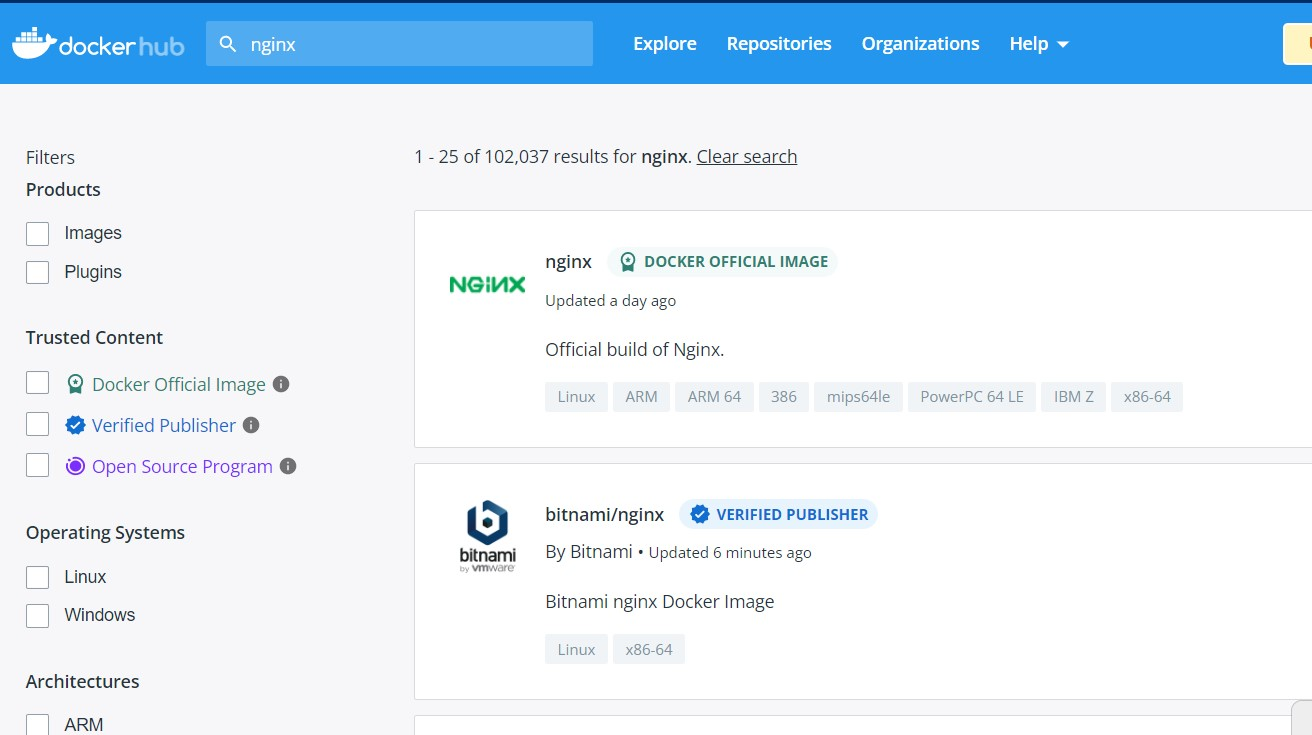
\includegraphics[scale=0.5]{fig15}
\caption{Nginx image on Docker hub}
\vspace{0.6\baselineskip}
\end{figure}	
 
 \item On the Docker Host, use the Docker pull command to download the latest nginx image from Docker Hub.
 
\begin{figure}[H]
\centering
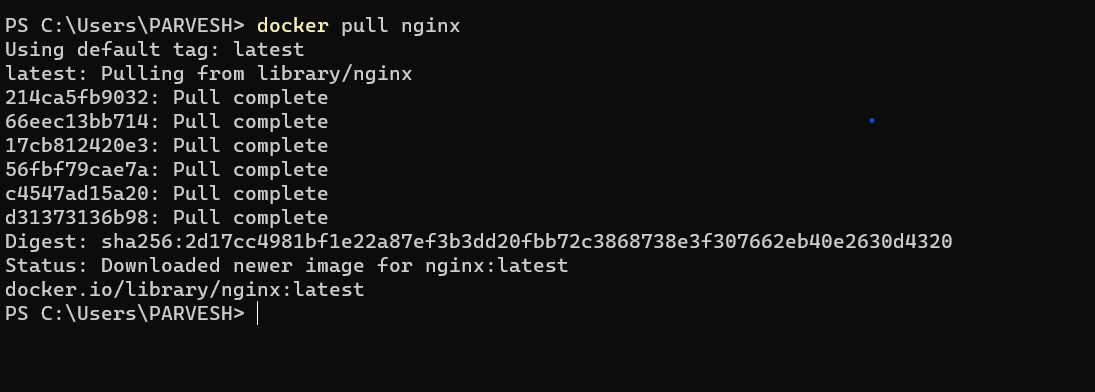
\includegraphics[scale=0.6]{fig16}
\caption{Pull nginx image}
\vspace{0.6\baselineskip}
\end{figure}	
 
 \item Now we have to run the NGINX image such that it will expose the Docker container port to the network port.
 
\begin{figure}[H]
\centering
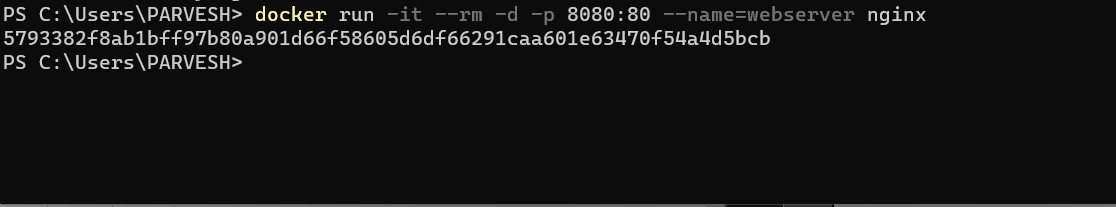
\includegraphics[scale=0.6]{fig17}
\caption{Run nginx image}
\vspace{0.6\baselineskip}
\end{figure}	

Here, we have used the -i and -t options to run the container interactively, the –rm option to delete the container on exit, -d option to run the container in the background or detached mode, and the –name option to provide a name to the container. Finally, we have provided the name of the Docker image that we want to pull. We have also used the -p option to publish port 8080 of the container to port 80 of the host machine. Let’s try to execute this command inside the terminal.

	\item Let’s verify by listing all the active containers.
	
\begin{figure}[H]
\centering
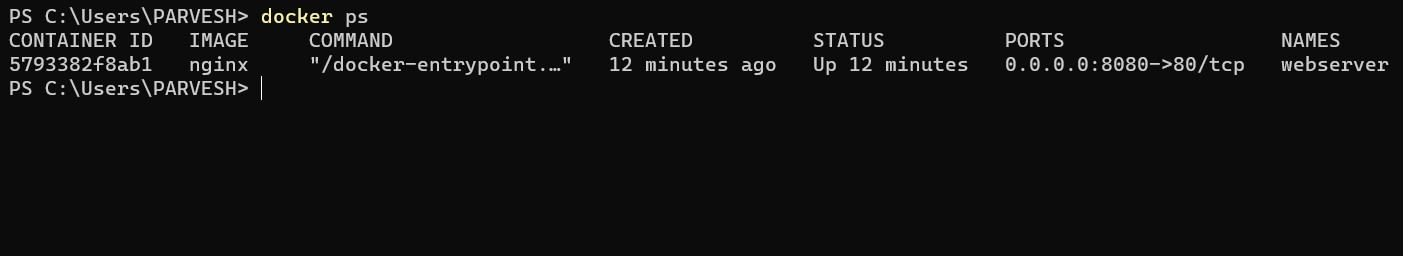
\includegraphics[scale=0.5]{fig18}
\caption{Listing running containers}
\vspace{0.6\baselineskip}
\end{figure}	

	\item To see that the container is actively running, navigate to the link localhost:8080 inside a browser, we will find the welcome page of the Nginx web server.
	
\begin{figure}[H]
\centering
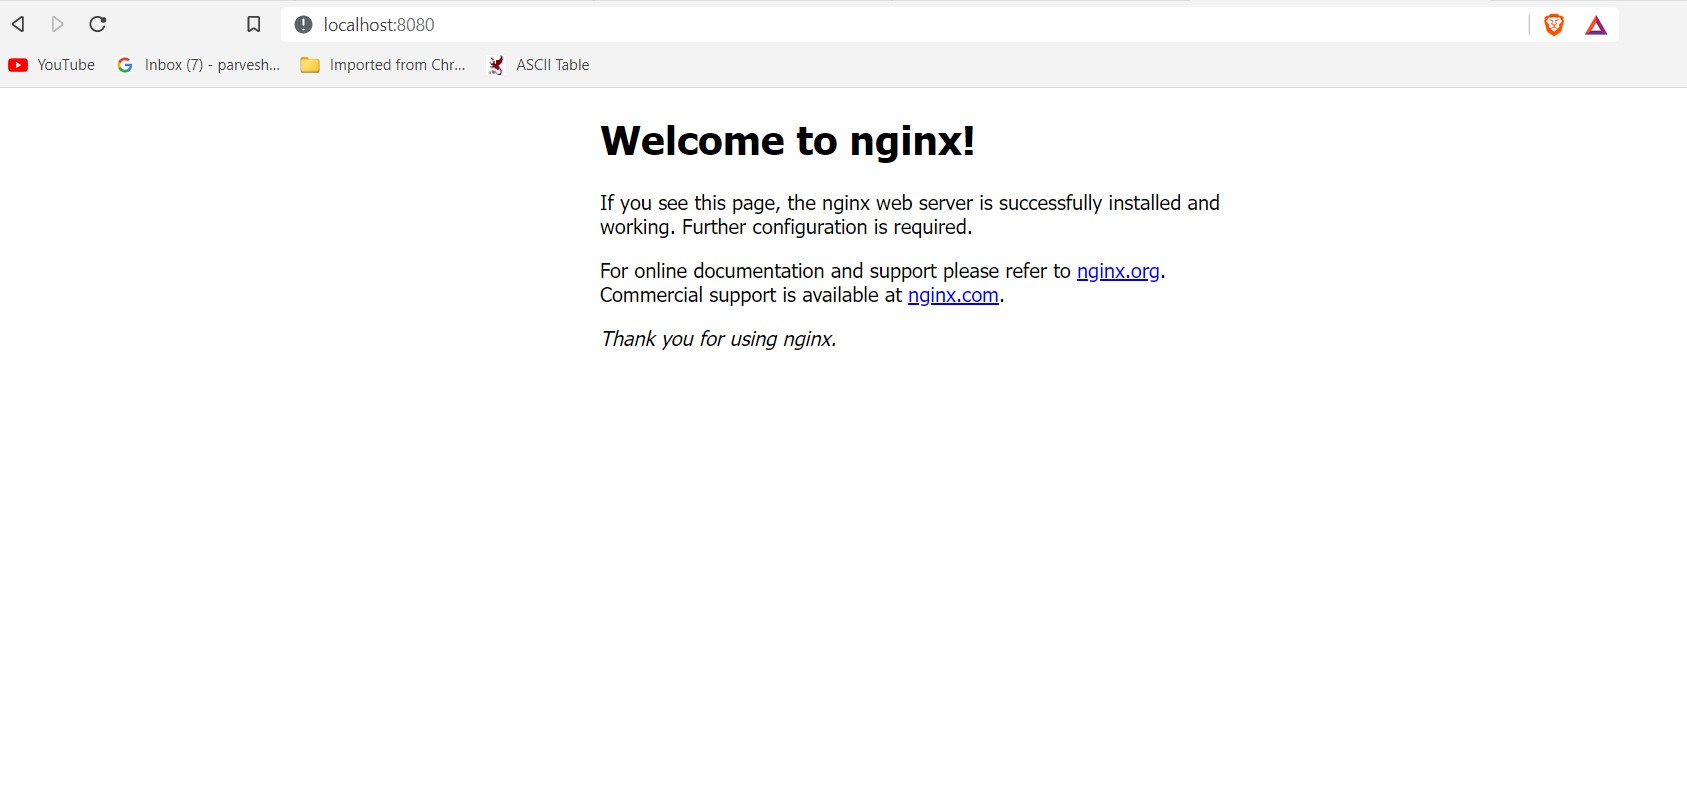
\includegraphics[scale=0.45]{fig19}
\caption{Nginx welcome page}
\vspace{0.6\baselineskip}
\end{figure}	
 
 \item To stop the container use the 'docker stop' command
 
\begin{figure}[H]
\centering
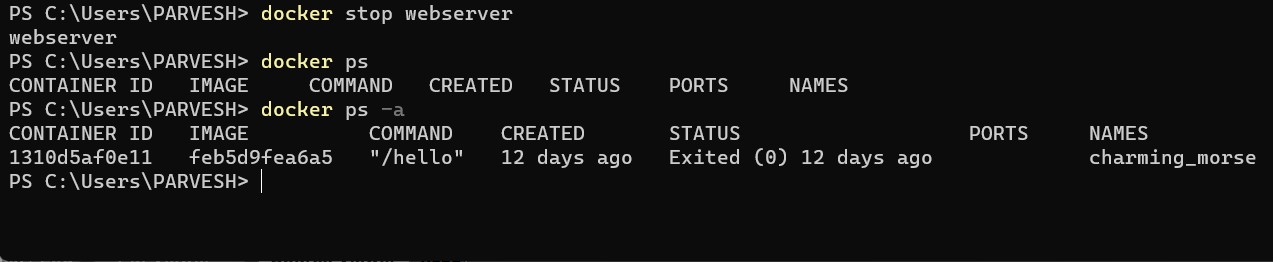
\includegraphics[scale=0.6]{fig20}
\caption{Stop Nginx}
\vspace{0.6\baselineskip}
\end{figure}	

 \end{enumerate}
 
 \clearpage


\section{PRACTICAL 7}

\textbf{\uppercase {Deploy Apache Web Server Image on Docker}} \\
\vspace{0.1\baselineskip} \\

Steps for getting the Docker container for Apache Web Server Image on Docker.

\begin{enumerate}
\item Log into Docker Hub, you will be able to search and see the image for apache as httpd.

\begin{figure}[H]
\centering
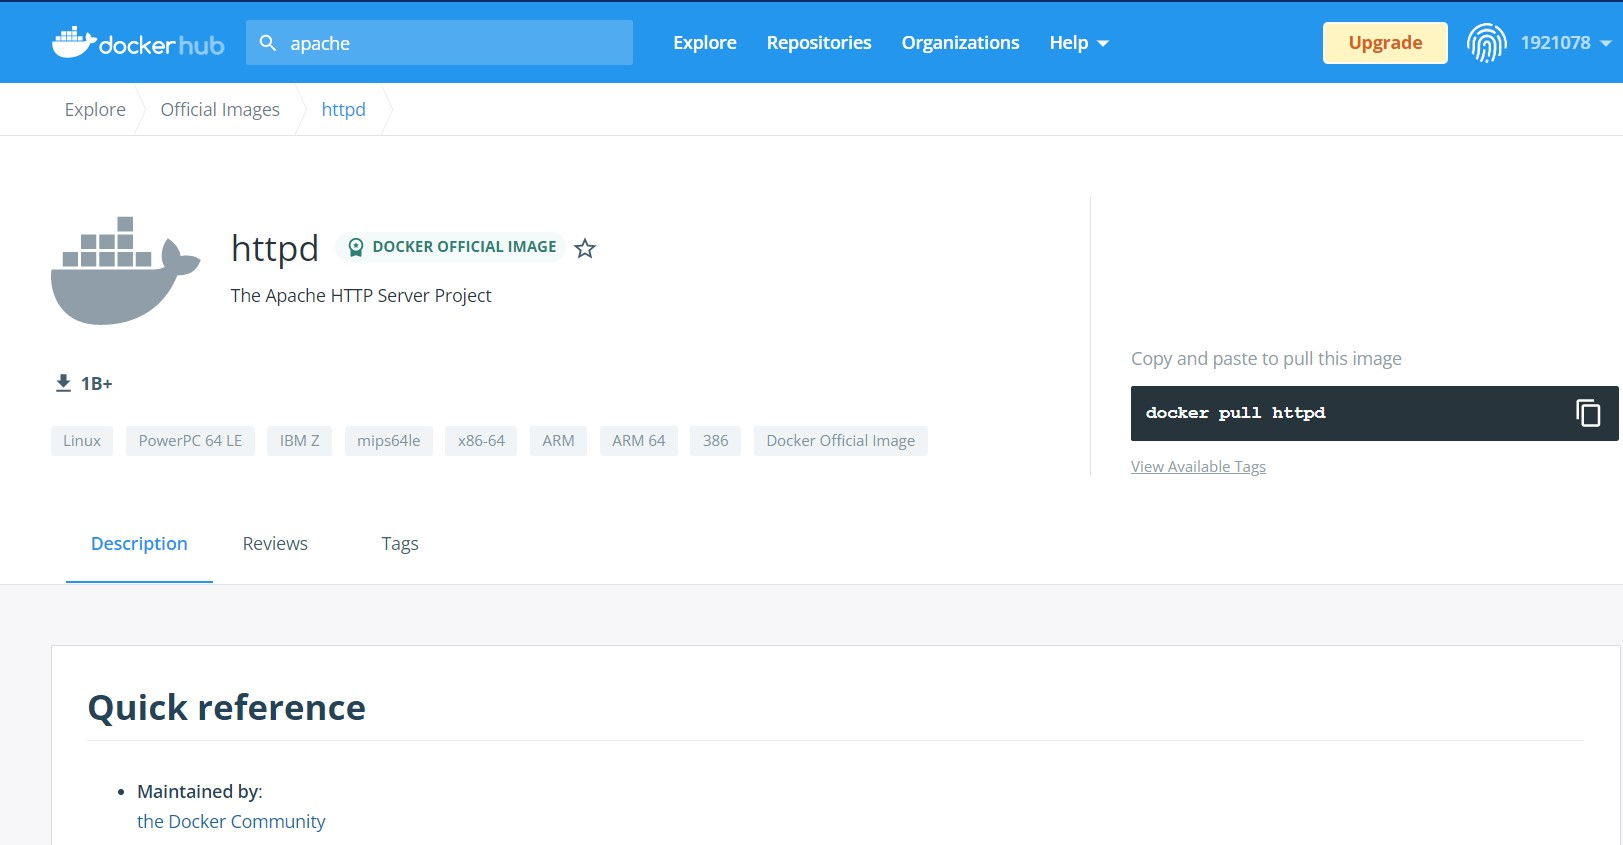
\includegraphics[scale=0.5]{fig21}
\caption{httpd Image On Docker Hub}
\vspace{0.6\baselineskip}
\end{figure}


\item Pull the Docker image, which contains Apache called httpd, by running the docker pull command below. This command will download or pull the Apache image from the Docker registry, as shown below.

\begin{figure}[H]
\centering
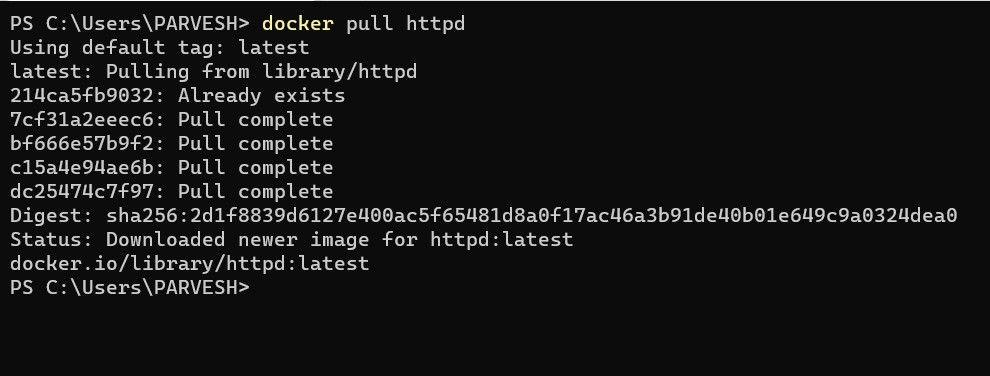
\includegraphics[scale=0.6]{fig22}
\caption{Pull httpd}
\vspace{0.6\baselineskip}
\end{figure}	

\item Next, confirm the downloaded image by running the docker images command below to list all images available on your computer.

\begin{figure}[H]
\centering
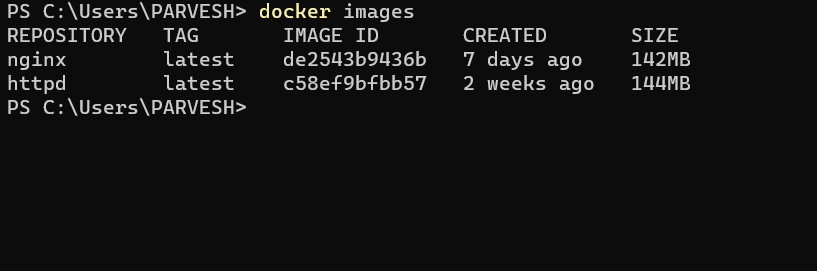
\includegraphics[scale=0.7]{fig23}
\caption{Check Images}
\vspace{0.6\baselineskip}
\end{figure}	

\item Invoke the docker run command to create a new container based on your downloaded Apache Docker image. The docker run command then returns the unique container ID of the container you’ve just created. Save this container id in the highlighted box below to the future if you wish to delete or remove the container.

\begin{figure}[H]
\centering
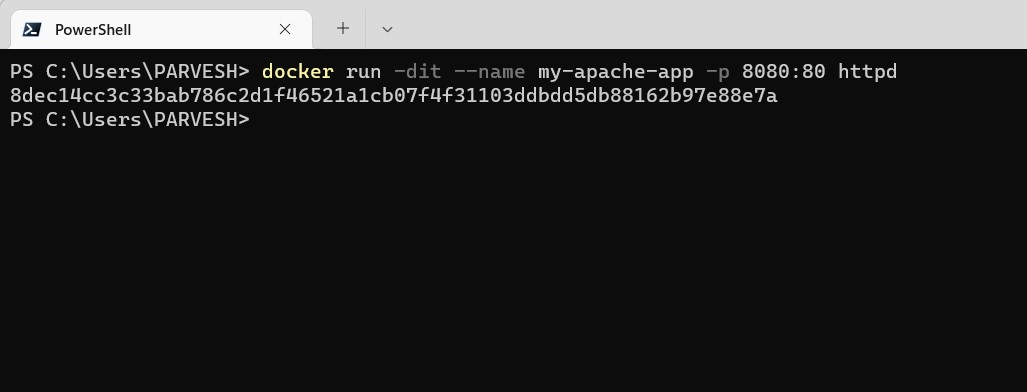
\includegraphics[scale=0.6]{fig24}
\caption{Run Server}
\vspace{0.6\baselineskip}
\end{figure}	

\item Once the Apache container is running, verify it by access the Apache web interface by navigating to Public-Ip-address:80 using any web browser. If you can see the same message, as you can see below, then you’ve successfully started your Apache Docker container.

\begin{figure}[H]
\centering
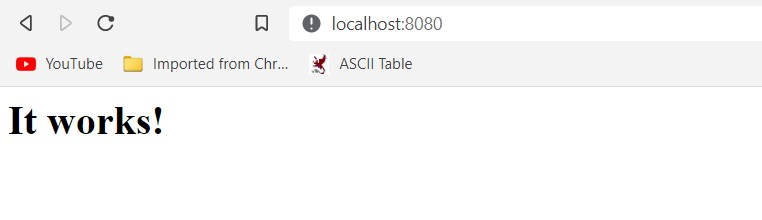
\includegraphics[scale=0.7]{fig25}
\caption{Default output of Apache web server}
\vspace{0.6\baselineskip}
\end{figure}	

\end{enumerate}

\clearpage


\section{PRACTICAL 8}

\textbf{\uppercase {Create Custom page using Web Server}} \\
\vspace{0.1\baselineskip} \\

\begin{enumerate}
\item First we create a running container. The docker create command will create a new container. Here we have requested a new container named baseimg with port 80 exposed to localhost. We are using nginx as a base image for the container. If you don’t have the nginx image in your local docker image repository, it will download automatically.

\begin{figure}[H]
\centering
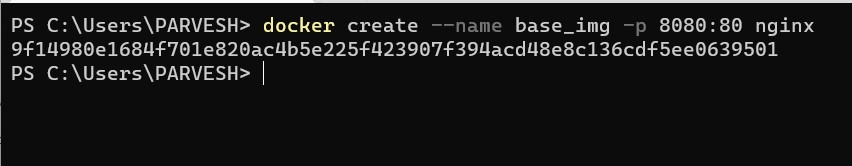
\includegraphics[scale=0.7]{fig26}
\caption{Creating a base container}
\vspace{0.6\baselineskip}
\end{figure}	

\item If you look at the list of images on your system, you will now see the nginx:alpine image.

\begin{figure}[H]
\centering
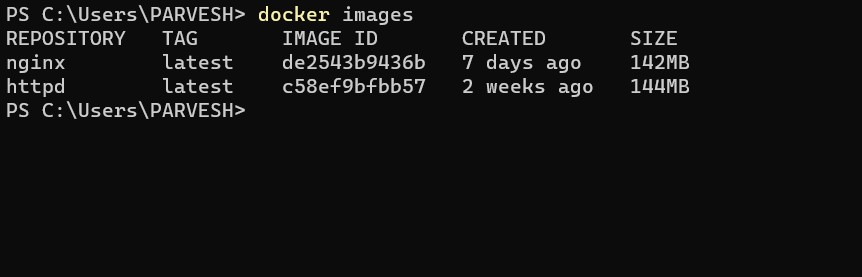
\includegraphics[scale=0.7]{fig27}
\caption{Inspect Images}
\vspace{0.6\baselineskip}
\end{figure}	


\item Note here that the container is not running, so you won’t see it in the container list unless you use the -a flag (-a is for all).

\begin{figure}[H]
\centering
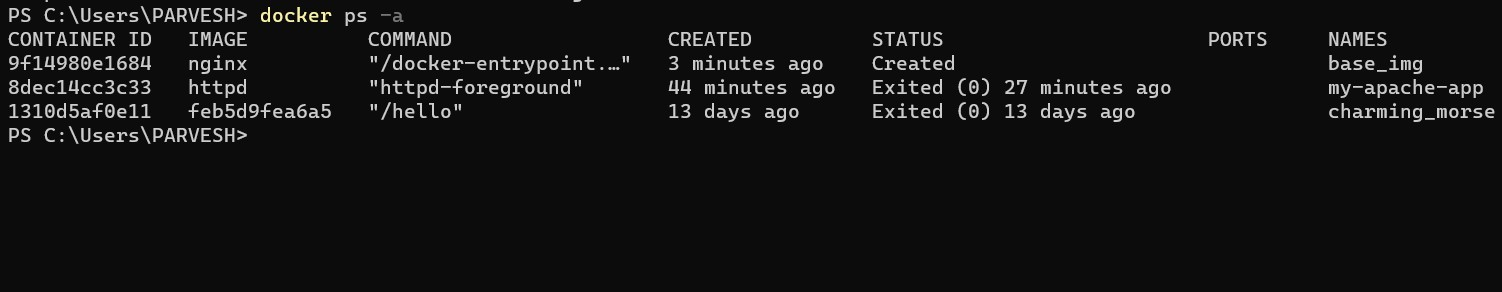
\includegraphics[scale=0.5]{fig28}
\caption{Inspect Container}
\vspace{0.6\baselineskip}
\end{figure}	

\item Start the container by running the following command.

\begin{figure}[H]
\centering
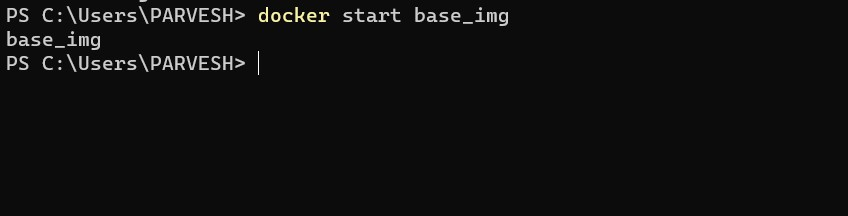
\includegraphics[scale=0.7]{fig29}
\caption{Start the container}
\vspace{0.6\baselineskip}
\end{figure}	

Now visit http://localhost with your browser. You will see the default “Welcome to nginx!” page. We are now running an nginx container.

\begin{figure}[H]
\centering
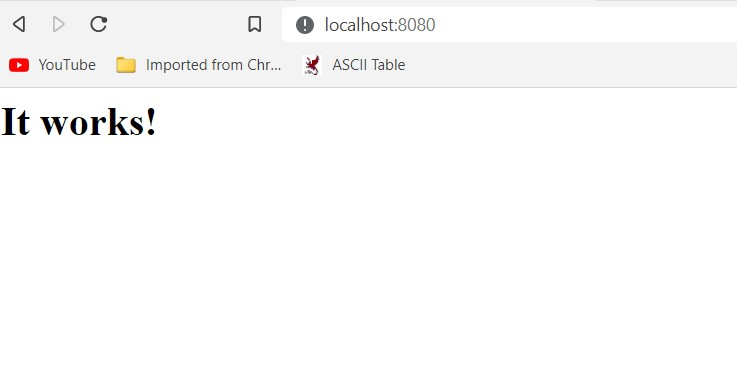
\includegraphics[scale=0.7]{fig30}
\caption{Container Running}
\vspace{0.6\baselineskip}
\end{figure}	

\item Let’s create a new index.html file and copy it onto the running container. Using an editor on your machine, create an index.html file in the same directory that you have been running Docker commands from. Then paste the following HTML into it:

\begin{figure}[H]
\centering
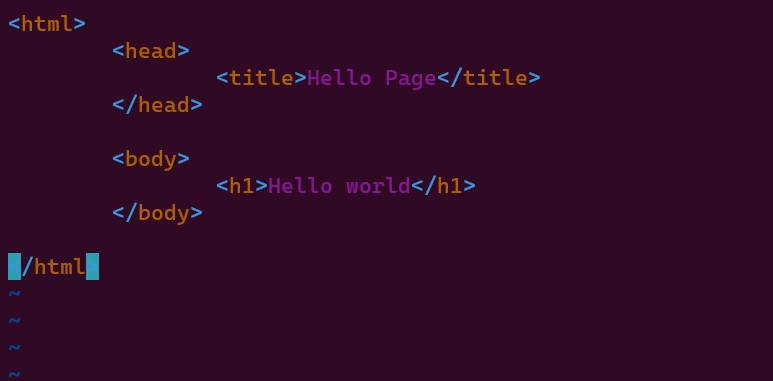
\includegraphics[scale=0.7]{fig31}
\caption{Html File}
\vspace{0.6\baselineskip}
\end{figure}	

\item Then save the file and return to the command line. We will use the docker cp command to copy this file onto the running container.

\begin{figure}[H]
\centering
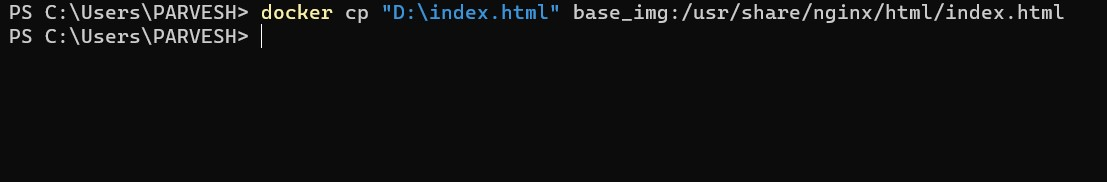
\includegraphics[scale=0.7]{fig32}
\caption{Copy file on running container}
\vspace{0.6\baselineskip}
\end{figure}	

\item Now reload your browser or revisit http://localhost. You will see the message “Hello World!” in place of the default nginx welcome page.

\begin{figure}[H]
\centering
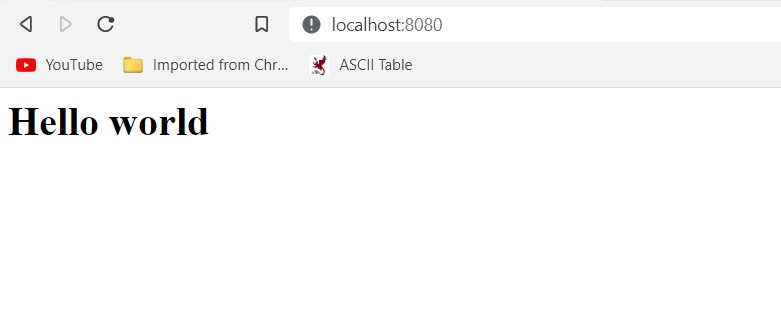
\includegraphics[scale=0.7]{fig33}
\caption{Modified page}
\vspace{0.6\baselineskip}
\end{figure}	


\end{enumerate}

\clearpage

\section{PRACTICAL 9}

\textbf{\uppercase {Create Custom image}} \\
\vspace{0.1\baselineskip} \\

Steps to Create a custom image 

\begin{enumerate}
\item First we have to create a directory named my-app and move into that directory and create a new empty file (Dockerfile).

\item write the following commands in Dockerfile.

\begin{figure}[H]
\centering
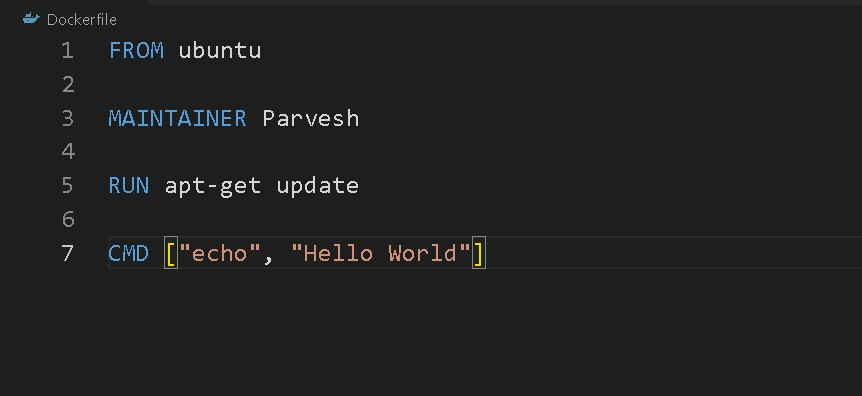
\includegraphics[scale=0.7]{fig34}
\caption{Dockerfile}
\vspace{0.6\baselineskip}
\end{figure}	

\item Save and exit the file.

\item You can check the content of the file by using the cat command.

\begin{figure}[H]
\centering
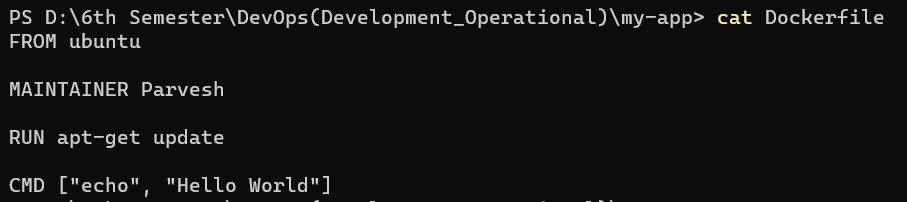
\includegraphics[scale=0.7]{fig35}
\caption{Checking content of Dockerfile}
\vspace{0.6\baselineskip}
\end{figure}	

\item The basic syntax used to build an image using a Dockerfile is: \textbf{\textit{docker build [OPTIONS] PATH | URL | -}}

\item Build a docker image,If you are already in the directory where the Dockerfile is located, put a . instead of the location. By adding the -t flag, you can tag the new image with a name which will help you when dealing with multiple images.

\begin{figure}[H]
\centering
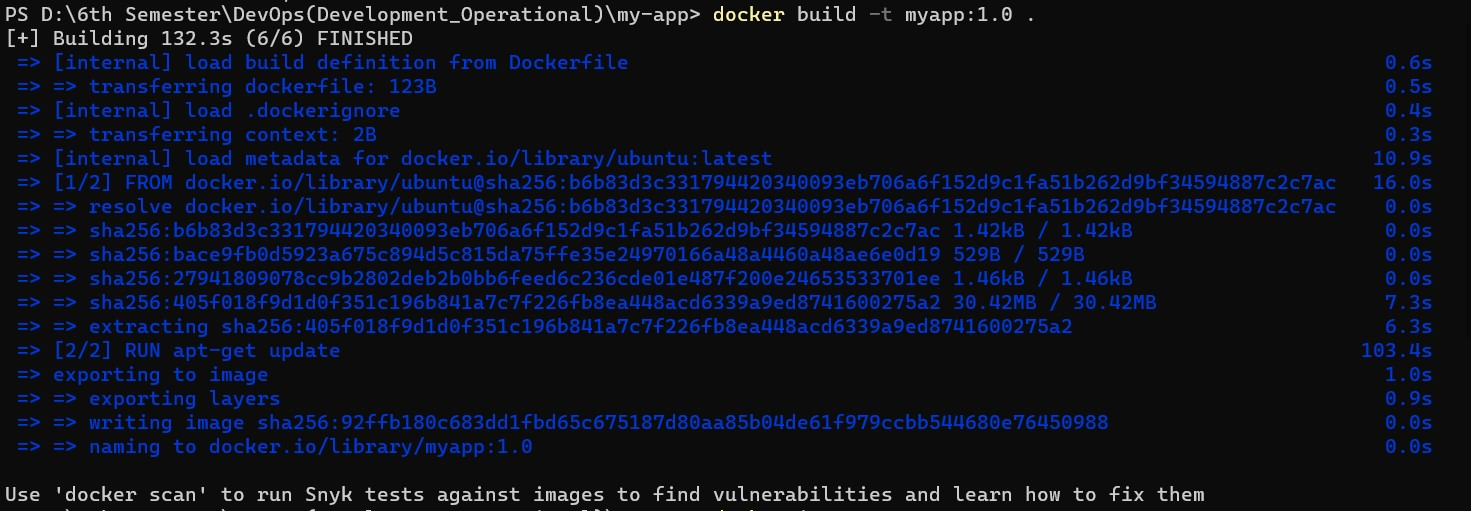
\includegraphics[scale=0.5]{fig36}
\caption{Building Image}
\vspace{0.6\baselineskip}
\end{figure}	


\item Once the image is successfully built, you can verify whether it is on the list of local images with the command.

\begin{figure}[H]
\centering
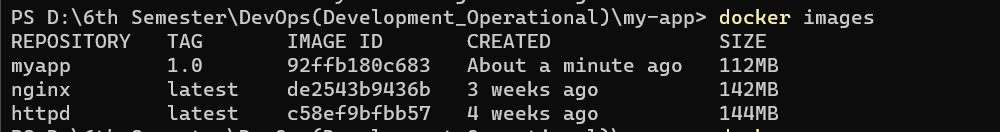
\includegraphics[scale=0.7]{fig37}
\caption{Verify image}
\vspace{0.6\baselineskip}
\end{figure}	

\item Launch a new Docker container based on the image you created in the previous steps.

\begin{figure}[H]
\centering
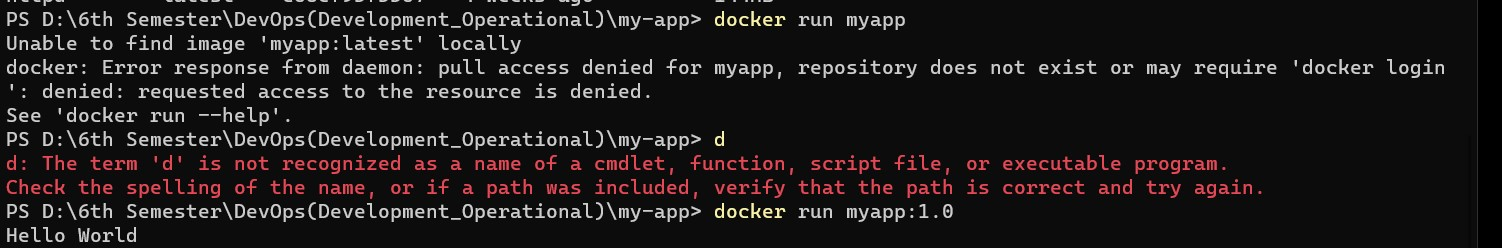
\includegraphics[scale=0.5]{fig38}
\caption{Launching Docker container}
\vspace{0.6\baselineskip}
\end{figure}	


\end{enumerate}

\clearpage

\section{PRACTICAL 10}

\textbf{\uppercase {Push Custom Image to Docker Hub}} \\
\vspace{0.1\baselineskip} \\

Steps to push a custom image  to Docker hub are: -

\begin{enumerate}

\item Docker images are pushed to Docker Hub through the docker push command. A single Docker Hub repository can hold many Docker images (stored as tags).


\item To create a repository, sign into Docker Hub, click on Repositories then Create Repository.

\begin{figure}[H]
\centering
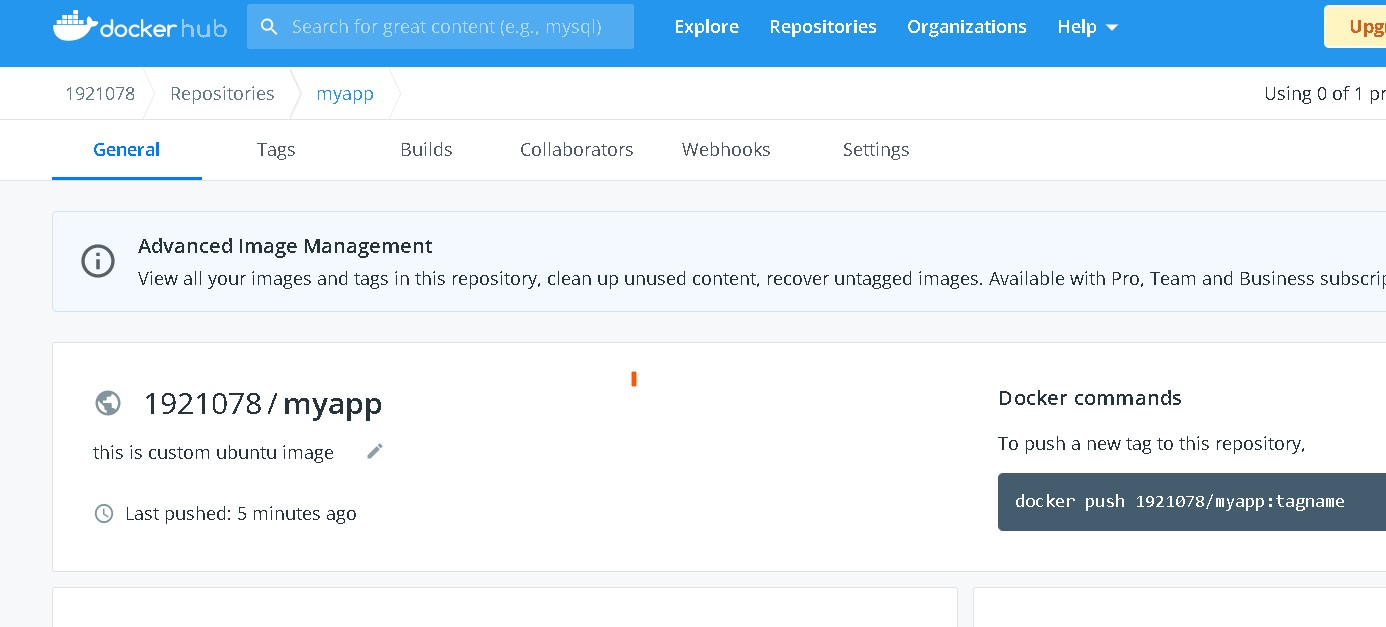
\includegraphics[scale=0.5]{fig39}
\caption{Create Repository}
\vspace{0.6\baselineskip}
\end{figure}	

\item To push an image to Docker Hub, you must first name your local image using your Docker Hub username and the repository name that you created through Docker Hub on the web.


\item Name your local images using  re-tagging an existing local image $ docker tag <existing-image> <hub-user>/<repo-name>[:<tag>]$

\begin{figure}[H]
\centering
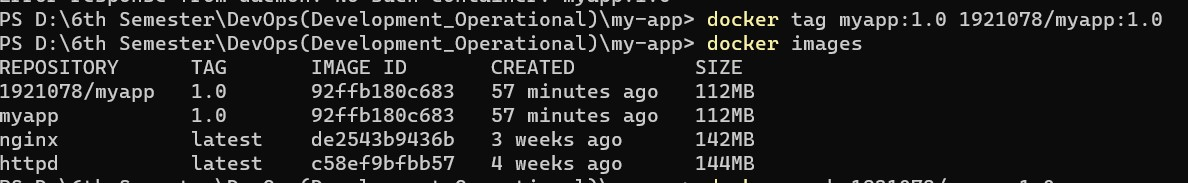
\includegraphics[scale=0.5]{fig40}
\caption{Re-tagging Repository}
\vspace{0.6\baselineskip}
\end{figure}

\item Push this repository to the registry designated by its name or tag.

\begin{figure}[H]
\centering
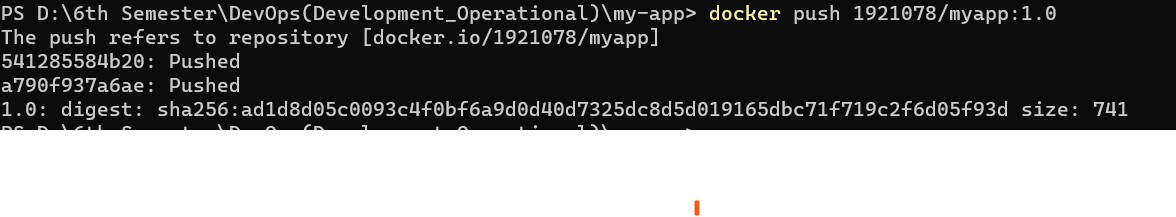
\includegraphics[scale=0.5]{fig41}
\caption{Push repository}
\vspace{0.6\baselineskip}
\end{figure}

\item The image is then uploaded and available for use by your teammates and/or the community.

\begin{figure}[H]
\centering
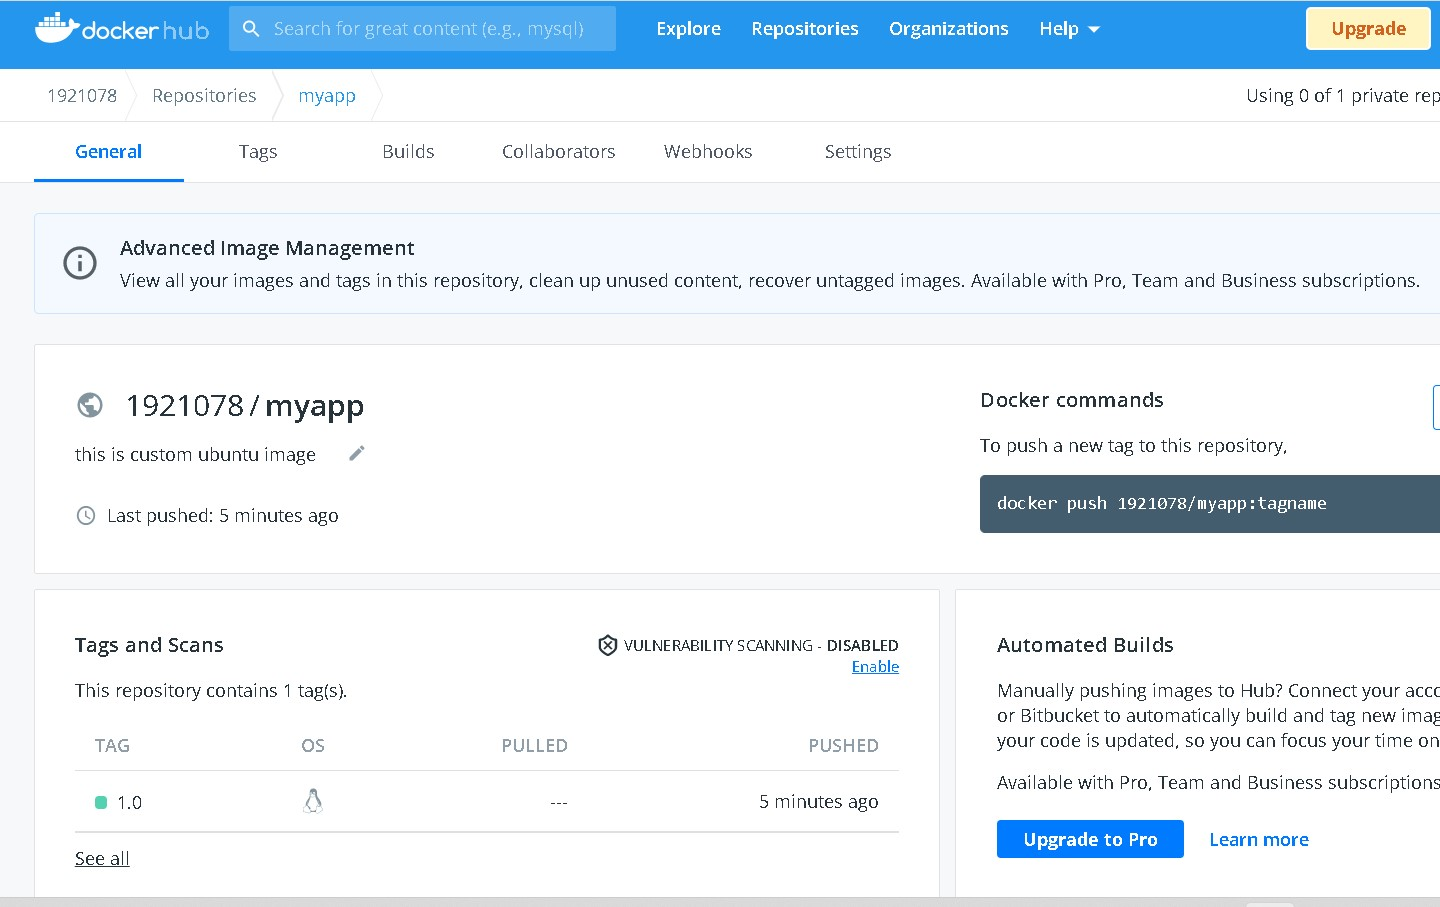
\includegraphics[scale=0.5]{fig42}
\caption{repository(Image) on Docker hub}
\vspace{0.6\baselineskip}
\end{figure}


\end{enumerate}


\clearpage

\section{PRACTICAL 11}

\textbf{\uppercase {Use Persistent storage with Docker}} \\
\vspace{0.1\baselineskip} \\

Docker has two options for containers to store files on the host machine, so that the files are persisted even after the container stops: volumes, and bind mounts.\\
Docker also supports containers storing files in-memory on the the host machine. Such files are not persisted. If you’re running Docker on Linux, tmpfs mount is used to store files in the host’s system memory. If you’re running Docker on Windows, named pipe is used to store files in the host’s system memory.

\begin{enumerate}
\item Volumes are stored in a part of the host filesystem which is managed by Docker (/var/lib/docker/volumes/ on Linux). Non-Docker processes should not modify this part of the filesystem. Volumes are the best way to persist data in Docker.

\item Bind mounts may be stored anywhere on the host system. They may even be important system files or directories. Non-Docker processes on the Docker host or a Docker container can modify them at any time.
\end{enumerate}


Steps to use Docker Volumes are: -

\begin{enumerate}
\item There are different ways to mount a Docker volume while launching a container. Users can decide between the -v and the --mount flags, which are added to the docker run command.

\item create a Docker volume.

\begin{figure}[H]
\centering
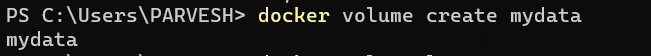
\includegraphics[scale=0.6]{fig43}
\caption{Create Volume}
\vspace{0.6\baselineskip}
\end{figure}

\item Verify you have successfully created a Docker volume, prompt Docker to list all available volumes.

\begin{figure}[H]
\centering
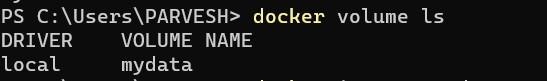
\includegraphics[scale=0.6]{fig44}
\caption{List volumes}
\vspace{0.6\baselineskip}
\end{figure}

\item To see more information about a Docker volume, use the inspect command.

\begin{figure}[H]
\centering
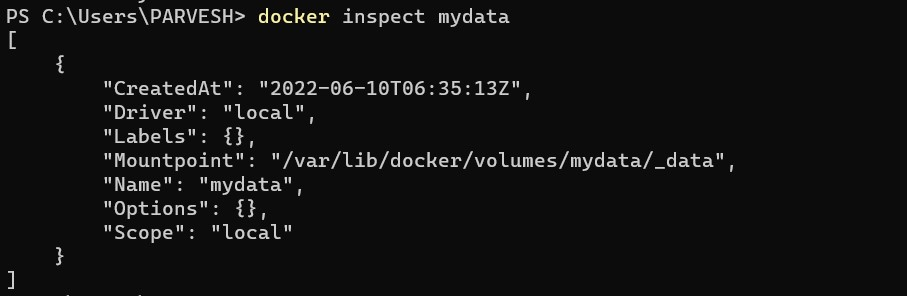
\includegraphics[scale=0.6]{fig45}
\caption{Inspect volume}
\vspace{0.6\baselineskip}
\end{figure}

\item To mount a data volume to a container add the --mount flag to the docker run command. It adds the volume to the specified container, where it stores the data produced inside the virtual environment. \\

To run a container and mount a data volume to it, follow the basic syntax:\\

$ docker run \--mount  source=[volume_name],destination=[path_in_container] [docker_image]$

\item  To launch an Ubuntu container and mount the mydata volume to it, run:\\

\begin{figure}[H]
\centering
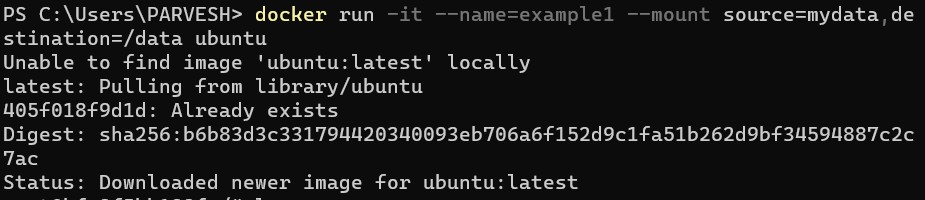
\includegraphics[scale=0.6]{fig46}
\caption{Mount mydata volume }
\vspace{0.6\baselineskip}
\end{figure}

The steps to Copying Files Between Containers From a Shared Volume are: -

\begin{enumerate}
\item  switched to the container command prompt, move to the data volume directory.

\item Create an empty sample file using the touch command.

\item Now, exit the container.

\begin{figure}[H]
\centering
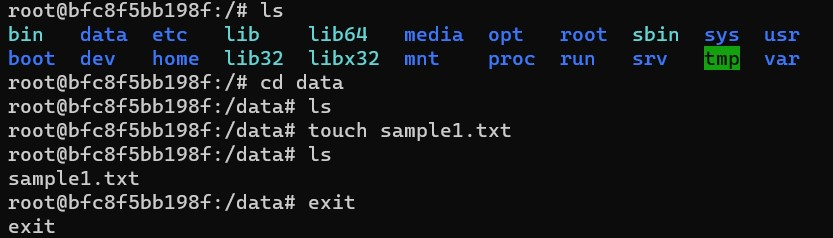
\includegraphics[scale=0.6]{fig47}
\caption{File in first container}
\vspace{0.6\baselineskip}
\end{figure}

\item Then, launch a new container example2 with the same data volume.

\begin{figure}[H]
\centering
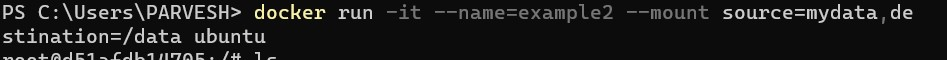
\includegraphics[scale=0.6]{fig48}
\caption{Launch example2 Container}
\vspace{0.6\baselineskip}
\end{figure}

\item List the content of the container. You should find the data directory, as in example1.

\item Move to the data directory and list the content of it.\\
The output should list the sample1.txt file you created in the previous container (example1).\\

\begin{figure}[H]
\centering
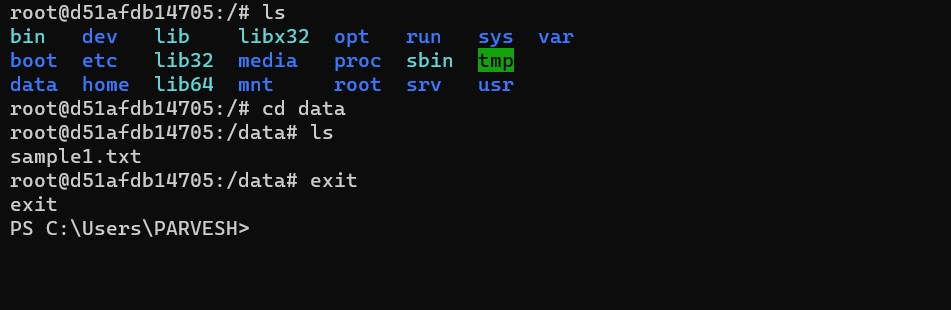
\includegraphics[scale=0.6]{fig49}
\caption{File in second container}
\vspace{0.6\baselineskip}
\end{figure}

\end{enumerate}

\end{enumerate}
You can also mount an existing directory from the host machine to a container. This type of volume is called Host Volumes.\\
You can mount host volumes by using the -v flag and specifying the name of the host directory.\\

The basic syntax for mounting a host directory is:\\
$docker run -v "\$(pwd)":[volume_name] [docker_image]$\\

The "\${pwd}" attribute instructs Docker to mount the directory the user is currently in.

The following example outlines how this is done.

\begin{enumerate}
\item First, create a sample directory on the host under the name tmp and move into it:

\item Once inside the directory, create a test file to see whether it will be available from the container.

\begin{figure}[H]
\centering
\includegraphics[scale=0.6]{fig50}
\caption{Sample Directory}
\vspace{0.6\baselineskip}
\end{figure}

\item Then, use the docker run command to launch an Ubuntu container with the host directory attached to it.

\item List the content of the container and verify there is a data1 directory.

\item Open the mounted directory and list the content. The output should display the file you created on the host.

\begin{figure}[H]
\centering
\includegraphics[scale=0.8]{fig51}
\caption{File in the container}
\vspace{0.6\baselineskip}
\end{figure}

\end{enumerate}


\end{document}
